\documentclass[24pt,pdf,xcolor=table]{beamer}
\usepackage{animate}
\mode<presentation>{}
\usepackage{graphicx}
\usepackage[export]{adjustbox}
\usepackage{subcaption}
\usepackage[utf8]{inputenc} 
\usepackage{beamerthemesplit}
\usetheme{Berlin}
\usecolortheme{dolphin}
\usepackage{enumerate}
\usepackage {tikz}
\usetikzlibrary{shadings}
\usetikzlibrary {positioning}
\usetikzlibrary{shapes.geometric}
\usepackage {xcolor}
\usepackage{hyperref}
\usepackage{ amssymb }
\usepackage{tcolorbox}
\usepackage{lipsum}
\usepackage{extarrows}% http://ctan.org/pkg/extarrows
\newcommand{\eqdef}{\xlongequal{\text{def}}}%
\hypersetup{
	bookmarksopen=false,
	pdfpagemode=UseNone,
	pdfpagemode=FullScreen,   
	pdfauthor={\textbf{Ahsanul Ameen(1605047)}} 
}

\definecolor {processblue}{cmyk}{0.96,0,0,0}


\title{Integer Linear Programming based approach}
\date{\today}



\begin{document}
	
\begin{frame}{\textit{ILP formulation and LP relaxation}}
	\titlepage
\end{frame}
	
%tableofContents  slide-1
\begin{frame}{Table of Contents}
	\tableofcontents
\end{frame}
	
\section{Set cover to ILP reduction}
\begin{frame}
  \begin{block}{Set cover}
    Input : $(U, S_1, S_2, \cdots, S_m)$
  \end{block}
  
  \begin{enumerate}
    \item introduce a variable $x_i$ for every set $S_i$
    \item $x_i$ = 1 when $S_i$ is selected, and $x_i$ = 0 otherwise.
  \end{enumerate}
\end{frame}


\begin{frame}{LP formulation}
	\begin{block}{derive the linear programming relaxation}
	  Minimize $\sum_{i = 1}^m x_i$
	  \newline Subject to 
	  \begin{itemize}
	    \item $\sum_{i:v \in S_i} x_i \ge 1$       $\forall v\in U$
	    \item $x_i \le 1$   $\forall i\in \{1, 2, \cdots, m\}$
	    \item $x_i \ge 0$   $\forall i\in \{1, 2, \cdots, m\}$
	  \end{itemize}
	\end{block}
\end{frame}	

\begin{frame}{Weighted LP optimization}
	\begin{block}{changing the cost method}
	  Minimize $\sum_{i = 1}^m w_i.x_i$
	  \newline Subject to 
	  \begin{itemize}
	    \item $\sum_{i:v \in S_i} x_i \ge 1$       $\forall v\in U$
	    \item $x_i \le 1$   $\forall i\in \{1, 2, \cdots, m\}$
	    \item $x_i \ge 0$   $\forall i\in \{1, 2, \cdots, m\}$
	  \end{itemize}
	\end{block}
\end{frame}	

\begin{frame}{Weighted LP optimization}
	\begin{block}{optimal fractional solution $x^*$}
	  $$x^*_i \in [0, 1]$$
	  we cannot round the $x^*_i$ to the nearest integer, because if an element $u$ belongs to $100$ sets, it could be
that $x^*_i$ = $\frac{1}{100}$ for each of those sets, and we would be rounding all those numbers to zero, leaving the element u not covered.
	\end{block}
\end{frame}	

\begin{frame}{Weighted LP optimization}
	\begin{block}{Simply rounding doesn't work here}
	  If we knew that every element u belongs to at most $k$ sets, then we could round the numbers $\ge \frac{1}{k}$ to $1$, and the numbers $\le \frac{1}{k}$ to zero.
	\end{block}
	\begin{block}{k - approximation}
	  Unfortunately, $k$ could be very large, even $\frac{n}{2}$
	\end{block}
\end{frame}	

\begin{frame}{Normalized Probability}
	\begin{block}{cosider $x^*_i$ as a probability}
	  we can think of the solution $x^*$ as describing a probability distribution over ways of choosing some of the subsets $S_1 , \cdots , S_m$, in which we choose $S_1$ with probability $x^*_1$ , $S_2$ with probability $x^*_2$ , and so on.
	\end{block}
\end{frame}	

\begin{frame}{Randomization}
	\begin{figure}[h]
		\centering
		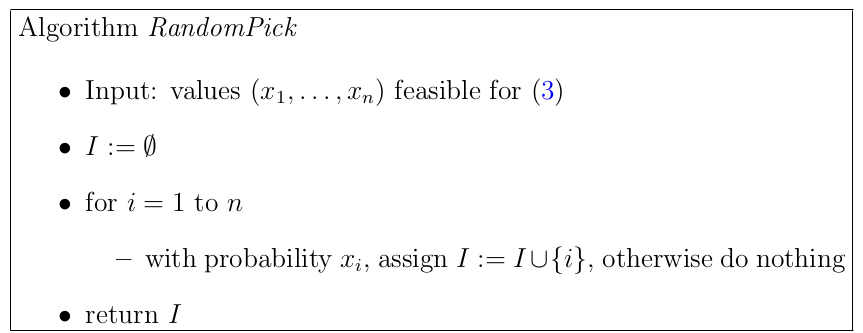
\includegraphics[width=1.0\textwidth]{./images/rp.png}
	\end{figure}
\end{frame}	

\begin{frame}{RandomPick}
	\begin{block}{Expected behaviour}
	  Using this probabilistic process, the expected cost of the sets that we pick is $i$ $\sum_{i = 1}^m w_i.x^*_i$,
	\end{block}
	
	\begin{block}{Expected behaviour}
	  Unfortunately, the solution that we construct could have a high probability of missing some of the elements
	\end{block}
\end{frame}
	
\begin{frame}{Randomization}
	\begin{figure}[h]
		\centering
		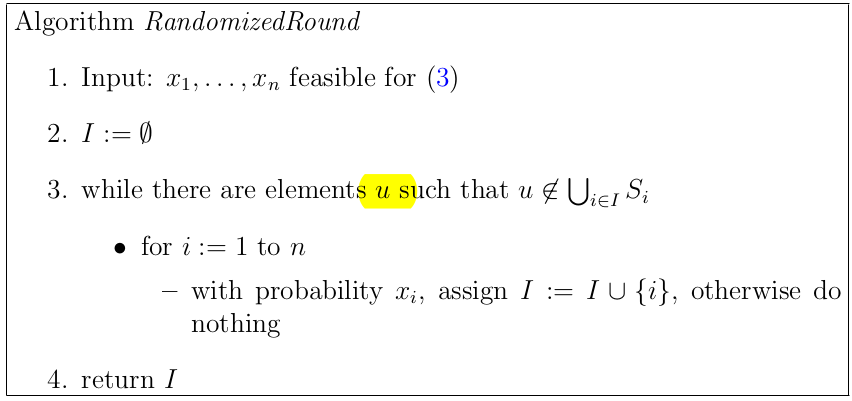
\includegraphics[width=1.0\textwidth]{./images/rr.png}
	\end{figure}
\end{frame}		
	
\begin{frame}{RandomidedRound}
	\begin{block}{Fact}
	  There is a probability at most $e^{-100}$ that the while loop is executed for more than $ln|U| + 100$ times. In general, there is a probability at most $e^{-k}$ that the while loop is executed form more than $ln|U| + k$ times.
	\end{block}
\end{frame}

\begin{frame}{RandomidedRound}
	\begin{block}{Fact}
	  Fix any positive integer parameter t and any feasible solution $(x_1, ..., x_m)$ for LP formulation. Then the expected size of $I$ in Algorithm RandomizedRound on input $(x_1, ..., x_m)$ after $t$ iterations. (or at the end of the algorithm, if it ends in fewer than $t$ iterations) is at most
	  $$t . \sum_{i=1}^m w_i.x_i $$
	\end{block}
\end{frame}


\begin{frame}{RandomidedRound}
	\begin{block}{Fact}
	  Given an optimal solution $(x^*_1, \cdots, x^*_m )$ to (3), algorithm RandomizedRound outputs, with probability $\ge .45$, a feasible solution to the set cover problem that contains at most $(2ln|U| + 6)$ · opt sets.
	\end{block}
\end{frame}

\end{document}
